\chapter{EEROS aktueller Stand}
\section{EEROS generell}
%TODO


\section{Aktuelle Implementierung des Sequencers}
Für EEROS besteht bereist ein rudimentärer \textit{Sequencer}.
Im folgenden Kapitel wird die bestehende Implementierung kurz erklärt.
In der Onlinedokumentation \cite{eerosOrg} wird noch vertiefter in die Details des bestehenden \textit{Sequencers} eingegangen, als in dieser Arbeit.


\subsection{Sequencer}
Die Grundlage bildet ein Sequencer-Objekt, das in einem Nicht-Realtime-Thread läuft.
In so einem \textit{Sequencer} können eine Serie von blockierenden \textit{Sequences} aufgerufen werden.
Wenn mehrere parallele \textit{Sequences} aufgerufen werden sollen, muss für jede \textit{Sequence} ein eigener \textit{Sequencer} erstellt werden.

\begin{figure}[!ht]
\centering
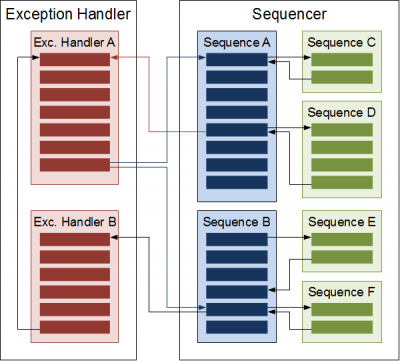
\includegraphics[angle=0,height=8cm]{images/SequencerBestehend.png}
\caption{Schematische Darstellung des bestehenden Sequencers \cite{eerosWiki}}
\label{sequencerBestehend}
\end{figure}


\subsection{Sequence}
Eine \textit{Sequence} führt als erstes eine benutzerdefinierte Initialisierungsfunktion aus.
Als nächstes wird eine \textit{preCondition} überprüft.
Fehlt die Überprüfung fehl, wird die \textit{Sequence} abgebrochen.
Bei einem positiven Ergebnis wird der Hauptteil, eine Abfolge von definierten \textit{Steps} ausgeführt.
Dem letzten \textit{Step} folgt noch eine Überprüfung einer \textit{postCondition}.
Läuft der \textit{Sequencer} im \textit{stepping-mode}, wird die \textit{Sequence} bei jeden \textit{yield()} pausiert und wird erst fortgeführt, wenn der Befehl dazu gegeben wird. \cite{eerosWiki}

\begin{lstlisting}
init();
yield();

if(!checkPreCondition()) 
  return SequenceResult<void>(result::preConditionFailure);
yield();

run();
yield();

if(!checkPostCondition())
  return SequenceResult<void>(result::postConditionFailure);
yield();

exit();
return SequenceResult<void>(result::success);
\end{lstlisting}


\subsection{Step}
Ein \textit{Step} ist eine vom \textit{Steuerungsentwickler} festgelegte Einheit, die von einem \textit{yield()} Befehl unterteilt wird.
\textit{Steps} können im \textit{stepping-mode} einzeln abgearbeitet werden.


\subsection{Sub-Sequence}
\textit{Subsequences} sind sehr ähnlich wie normale \textit{Sequenzen}.
Sie können verwendet werden, wenn ein ähnlicher Ablauf mehrmals wiederholt werden soll.
Durch eine Übergabe von Parameter an eine solche \textit{Subsequence} kann sie sehr flexibel gestaltet werden.
Wenn die \textit{Subsequence} parallel, also nicht-blockierend, aufgerufen werden soll, muss sie einem neuen Sequencer übergeben werden.

\begin{lstlisting}
class SequenceB : public Sequence<> {
public:
  SequenceB(std::string name, Sequencer* seq, Robot& r) : Sequence<void,double>(name, seq), robot(r){ }
 
  void run() {
    robot.moveZ(5);
    sleep(3);
    yield();
    robot.moveZ(0);
  }
 
private: 
  Robot& robot;
};
\end{lstlisting}


\subsection{Error-Handler}
Der \textit{Error-Handler} wird in der Onlinedokumentation zwar erwähnt, im Sourcecode von EEROS sind aber keine Spuren von der Implementierung zu finden.
Der Dokumentation zu folge soll er \textit{Exceptions} behandeln.
Je nach \textit{Exception} soll er flexibel reagieren, um Probleme zu beheben.



%\section{Fallbeispiel Parallel Scara}
%
%\begin{figure}[!ht]
%\centering
%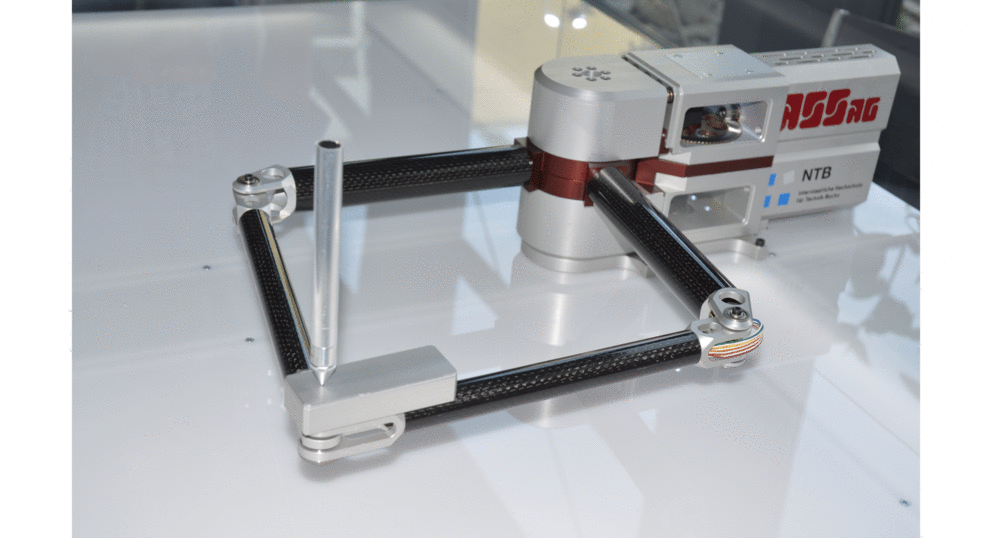
\includegraphics[angle=0,height=8cm]{images/ParallelScara.png}
%\caption{Der Parallel Scara Roboter \protect\footnote{http://www.ntb.ch/projekt/parallel-scara/}}
%\label{parallelScara}
%\end{figure}
%
%Der Parallel Scara ist ein Roboter, dessen Hardware und auch Software an der NTB entwickelt wurde.
%Die Steuerung ist mit EEROS und dem bestehenden \textit{Sequencer} aufgebaut.
%Im folgenden Kapitel wird der Quellcode der Steuerung analyisiert um herauszufinden, welche Aspekte des bestehenden \textit{Sequencers} brauchbar sind, und wo er noch Lücken aufweist.
%
%
%\subsection{asdf}



\section{Fallbeispiel 'EEDURO Delta Roboter'}

%\begin{figure}[!ht]
%\centering
%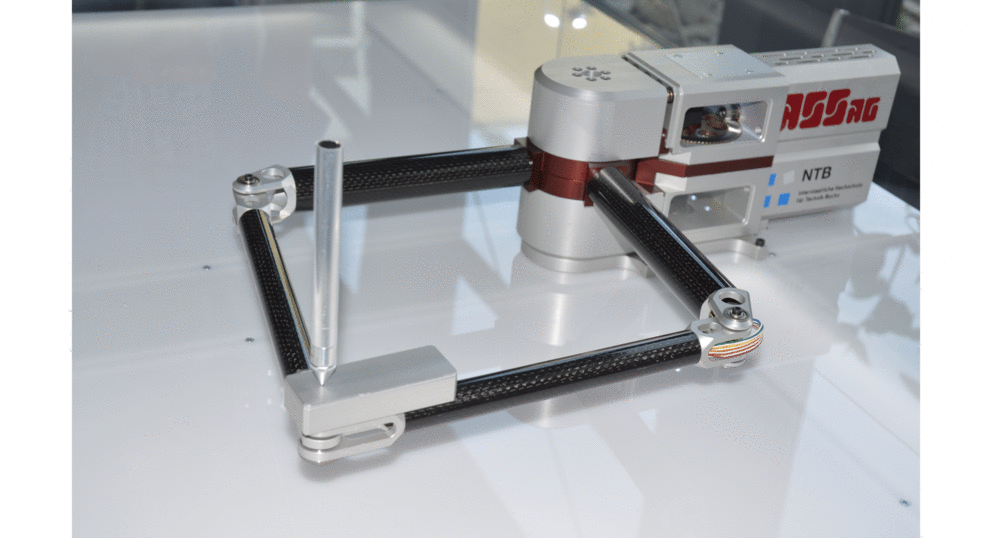
\includegraphics[angle=0,height=8cm]{images/ParallelScara.png}
%\caption{Der Parallel Scara Roboter \protect\footnote{http://www.ntb.ch/projekt/parallel-scara/}}
%\label{parallelScara}
%\end{figure}

Der \textit{EEDURO Delta Roboter} ist ein Roboter, dessen Hardware und auch Software an der NTB entwickelt wurde.
Die Steuerung ist mit EEROS und dem bestehenden \textit{Sequencer} aufgebaut.
Im folgenden Kapitel wird der Quellcode der Steuerung analyisiert um herauszufinden, welche Aspekte des bestehenden \textit{Sequencers} brauchbar sind, und wo er noch Lücken aufweist.

Der Quellcode der Steuerungssoftware ist auf folgendem Git-Repository zu finden: \\
\textit{https://github.com/ClaudiaVisentin/eeduro-platform }

%Die Software wurde vom Stand 10.10.2016 mit folgendem Hashverwendet: \\ \textit{a25bcfa752516723f067f5a5166e8f09e60fc6e8}
Die Software wurde vom Stand 10.10.2016 mit dem Hash \textit{\seqsplit{a25bcfa752516723f067f5a5166e8f09e60fc6e8}} verwendet.


\subsection{asdf}
